%----------------------------------------------------------------------------------------
%	PACKAGES AND OTHER DOCUMENT CONFIGURATIONS
%----------------------------------------------------------------------------------------
\documentclass[margin, centered]{res}
\topmargin=-0.5in
\oddsidemargin -.5in
\evensidemargin -.5in
\textwidth=6.5in
\itemsep=0in
\parsep=0in
\newsectionwidth{1in}
\usepackage[pdftex]{graphicx}
\usepackage{enumitem}
\usepackage{wrapfig}
\usepackage{helvet}
\usepackage[colorlinks = true,
            linkcolor = black,
            urlcolor  = black,
            citecolor = black,
            anchorcolor = black]{hyperref}
\setlength{\textwidth}{6.5in} % Text width of the document
\setlength{\textheight}{720pt}

\begin{document}

%----------------------------------------------------------------------------------------
%	NAME AND ADDRESS SECTION
%----------------------------------------------------------------------------------------\
\setlength{\voffset}{0.75in}
\begin{center}
    \hspace{-\hoffset}
    \huge\bf{\href{https://www.hridaydutta123.github.io}{Hridoy Sankar Dutta}}
    \hfill 
\smash{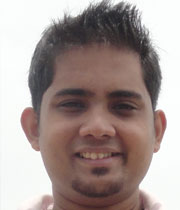
\includegraphics[width=3cm]{hridoyd.jpg}}
\end{center}
\vspace{-5mm}
\moveleft\hoffset\vbox{\hrule width 19cm height 0.5pt}
\vspace{-7mm}
\begin{center}
    \hspace{-\hoffset}
    \href{mailto:hridaydutta123@gmail.com}{hridaydutta123@gmail.com} ~\textbullet~ \(+91\)8638189794 ~\textbullet~ \#3-E, Pink Enclave, Paltan Bazar, Guwahati, Assam - 781008
\end{center}
\vspace{-7mm}
\begin{resume}
\section{Links}
\textbf{Website:} \url{https://hridaydutta123.github.io} \\
\textbf{Github:} \url{https://github.com/hridaydutta123/} \\
\textbf{DBLP:} \url{http://dblp.uni-trier.de/pers/hd/d/Dutta:Hridoy_Sankar} \\
\textbf{Google Scholar:} \url{https://scholar.google.co.in/citations?user=4UrQjwUAAAAJ&hl=en} \\
\textbf{Hackerearth:} \url{https://www.hackerearth.com/@hridaydutta123} \\
\textbf{LinkedIn:} \url{https://www.linkedin.com/in/hridoy-sankar-dutta-18448a63/?ppe=1} \\


%----------------------------------------------------------------------------------------
%	EDUCATION SECTION
%----------------------------------------------------------------------------------------
\section{Education}
\textbf{PhD in Computer Science and Engineering} \hfill 2017 - Present \\
\href{http://www.iiitd.ac.in/}{Indraprastha Institute of Information Technology Delhi (IIIT-D), India}
\begin{itemize}
 \item Supervisor: Dr. Tanmoy Chakraborty, Assistant Professor \& Ramanujan Fellow, Indraprastha Institute of Information Technology Delhi (IIIT-D), India
\end{itemize}
\textbf{M.Tech in Computer Science and Engineering} \hfill 2015 - 2017 \\
\href{http://www.nitdgp.ac.in/}{National Institute of Technology Durgapur, West Bengal, India}
\begin{itemize}
 \item CGPA of \textbf{9.15}/10 (May 2017)
\end{itemize}
\textbf{B.Tech in Computer Science and Engineering} \hfill 2009 - 2013 \\
\href{http://www.gauhati.ac.in/}{Institute of Science and Technology, Gauhati University, Assam, India}
\begin{itemize}
 \item CGPA of \textbf{9.17}/10 (May 2013)
\end{itemize}
\textbf{High School} - \href{http://www.ssa-school.org/}{Shrimanta Shankar Academy, Guwahati} (CBSE) - \textbf{82.80\%} \hfill 2007 - 2009 \\
\textbf{Secondary School} - Hindustani Kendriya Vidyalaya (CBSE) - \textbf{81.00\%} \hfill 2000 - 2007
 
%----------------------------------------------------------------------------------------
%	WORK EXPERIENCE SECTION
%----------------------------------------------------------------------------------------
\section{Job Experience}
\textbf{Assistant Project Engineer, IIT Guwahati} \hfill Aug, 2014 - Apr, 2015\\
Developing Text to Speech System in Assamese Language Phase II. \\

%----------------------------------------------------------------------------------------
%	OTHER EXPERIENCES SECTION
%----------------------------------------------------------------------------------------
\section{Other Experiences}
\textbf{Student Researcher, ForkIT} \\
\emph{Mentored by {Dr. Subrata Nandi, Dept. of CSE, NIT Durgapur} \& \\ {Dr. Sujoy Saha, Dept. of CSE, NIT Durgapur}} \hfill May, 2016 - June, 2017 \\
An End-to-end system to generate Offline Crisis maps \\
\\
\textbf{Summer Research Intern in DISARM Group, NIT Durgapur} \\
\emph{Mentored by {Dr. Subrata Nandi, Dept. of CSE, NIT Durgapur}} \hfill May, 2016 - July, 2016 \\
Developed web application Admin Dashboard for Master Control Station at the time of disaster. Django, a python web framework was used to develop the application.\\
\\
\textbf{Winter Research Intern in DISARM Group, NIT Durgapur} \\
\emph{Mentored by {Dr. Subrata Nandi, Dept. of CSE, NIT Durgapur}} \hfill Dec, 2015 - Jan, 2016 \\
Developed an Oppurtunistic Network for Android Application.
\\
\\
\textbf{Project Intern, IIT Guwahati}  \\
\emph{Mentored by {Dr. Sushanta Karmakar, Dept. of CSE, IIT Guwahati}} \hfill Jan, 2013 - June, 2013 \\
Worked on the Research Topic "Hierarchical topology adaptation for distributed convergecast applications"
\\
\\
\textbf{Summer Trainee, \href{http://neepco.co.in/neepco/}{NEEPCO}} \\
\emph{Mentored by {Subhash Kalita, Manager(System)}} \hfill June, 2012 - July, 2012 \\
Developed a e-File Sharing System among the users of the organization. PHP language was used to develop the application.
\\
\\
\newpage
\textbf{Summer Trainee, \href{http://amtron.in/}{AMTRON}}  \\
\emph{Mentored by {SD \& P Divn., AEDC Ltd.}} \hfill June, 2011 - July, 2011 \\
MS Access Form Management.
\\
\\

%----------------------------------------------------------------------------------------
%	TECHNICAL SKILLS SECTION
%----------------------------------------------------------------------------------------

\section{Technical \hspace{2mm} Skills}
\textbf{Strongest Areas} - Data Structures, Databases, Algorithms, Web Technology \\
\textbf{Languages} - Java, Python,  PHP, C++, UNIX Shell, HTML, CSS, JS, Ajax, Perl, Responsive Design \\
\textbf{Frameworks} - Django, Flask, Phonegap \\
\textbf{Tools} - Git, Android Studio, Adobe Photoshop, JUnit, \LaTeX \\
\textbf{Databases} - MySQL, SQLite \\

%---------------------------------------------------------------------------------------
%	PUBLICATION SECTION
%---------------------------------------------------------------------------------------

\section{Publications}
\begin{itemize}[leftmargin=*]
\item Partha Sarathi Paul, \textbf{Hridoy Sankar Dutta}, Bishakh Chandra Ghosh, Krishnandu Hazra, Sandip Chakraborty, Sujoy Saha, Subrata Nandi, ``Offline crisis mapping by opportunistic dissemination of crisis data after large-scale disasters'', Proceedings of the Second ACM SIGSPATIAL International Workshop on the Use of GIS in Emergency Management.
\item Sandip Chakraborty, Suchetana Chakraborty, Sushanta Karmakar, \textbf{Hridoy Sankar Dutta}, ``Hierarchical topology adaptation for distributed convergecast applications'', Proceedings of the 29th Annual ACM Symposium on Applied Computing.
\end{itemize}

%----------------------------------------------------------------------------------------
%	RELEVANT COURSE SECTION
%----------------------------------------------------------------------------------------
\section{Certified \hspace{2mm} Courses}
\begin{itemize}[leftmargin=*]
\item \textbf{JAVA} Programming Course at InfoConnect Solutions \hfill Aug, 2011 - Feb, 2012 \\
\end{itemize}
%----------------------------------------------------------------------------------------
%	Selected Projects Section
%----------------------------------------------------------------------------------------
\section{Selected Projects}
All projects available on git : \url{https://www.github.com/hridaydutta123}
%\setlist[itemize]{
\begin{itemize}[leftmargin=*]
 \item \textbf{\href{https://github.com/Bug-Assassins/DFC_query_builder}{Opportunistic Network for Android Application}} - Implementation of Communication Medium for Challenge Network Scenario. Opportunistic network offers many appealing application perspectives from local social-networking applications to supporting communications in remote areas or in disaster and emergency situations. Communication medium will automatically work as hotspot or wifi mode depending upon the environmental scenario.
 \item \textbf{\href{http://www.github.com/hridaydutta123/offlinemcs}{Offline Master Control Station}} - Implementation of reliable and effective data transfer from oppurtunistic network and tool for analyzing behaviour of data captured in Oppurtunistic Networks.
 \item \textbf{\href{http://www.iitg.ernet.in/cseweb/tts/tts/Assamese/}{Designing TTS System in Assamese and Manipuri Languages}} - It involves building systems for synthesizing natural speech in native Assamese and Manipuri tone from a 	given text and building user friendly GUIs for the common people.
 \item \textbf{\href{https://github.com/hridaydutta123/MapDisarm}{MapDisarm}} - Offline efficient transfer of OSM Map tiles among various devices without internet connectivity for gps based recovery in Oppurtunistic network.
 \item \textbf{\href{https://github.com/hridaydutta123/MapDisarm}{e-File Sharing System}} - Complete file management system for NEEPCO organization.
\end{itemize}

%----------------------------------------------------------------------------------------
%	ACHIEVEMENT SECTION
%----------------------------------------------------------------------------------------
\section{Achievements and Awards}
\begin{itemize}[leftmargin=*]
 \item Grand Challenge Grade \textbf{A} winner where smart \& embedded device innovators around the world vied for the top spot. Organised by International Symposium Embedded Devices, 2016 at IIT Patna.
 \item Came \textbf{1st Runners Up} in Startup Weekend, Kolkata (5-7th August, 2016).
 \item Media Coverage of our Group in a local daily: \url{http://aamarkatha.com/?p=1121#.WMzJSszEghE.whatsapp}
 \item Won \textbf{3rd Prize in Coding Competition} at Techniche 2012 ( IIT Guwahati Technical Fest Coding Event ).
 \item Attended NASSCOM Product Conclave-2016 as Student Researcher of ForkIT
 \item Rank of \textbf{3} in Master Of Technology.
 \item Rank of \textbf{7} in Bachelor Of Technology.
 \item Secured 10/10 SGPA in M.Tech(3rd \& 4th Semester)
 \item Secured 10/10 SGPA in B.Tech(6th,7th \& 8th Semester)
 \newpage
 \item GATE Qualified (2016) – \textbf{Gate Score : 488 ( AIR – 4370 ) }
 \item GATE Qualified (2015) – \textbf{Gate Score : 441 ( AIR – 6675 ) }
 \item Recipient of GATE Scholarship (2014) – \textbf{Gate Score : 582 ( AIR – 2139 ) }

 \item Passed “A” level examination of National Cadet Crops (NCC).
 \item Winner of Counter Strike Gaming Competition at Technoshine 2015, Technoshine 2016, Aarohan 2017 and Rectasy 2017 held at NIT Durgapur.
\end{itemize}


%----------------------------------------------------------------------------------------
%	ATTENDED EVENTS SECTION
%----------------------------------------------------------------------------------------
\section{Events \& Workshops Attended}
\begin{itemize}[leftmargin=*]
\item Workshop on Complex and Social Networks, IIT Kharagpur (2017)
\item NASSCOM Product Conclave, Bangalore (2016)
\end{itemize}

%----------------------------------------------------------------------------------------
%	HOBBIES SECTION
%----------------------------------------------------------------------------------------

\section{Hobbies}
Handling Systems, Trying Open-Source Softwares

\section{More}
Please visit \href{https://hridaydutta123.github.io}{https://hridaydutta123.github.io}

\end{resume}
\end{document}